\documentclass[a4paper]{article}

%--------------------------------------------------------------------------
\usepackage[a4paper, total={6in, 9in}]{geometry}
\usepackage{amsmath}
\usepackage{booktabs}
\usepackage{caption}
\usepackage{enumitem}
\usepackage{graphicx}
\usepackage{float}
\usepackage{inconsolata}
\usepackage{listings}
\usepackage{pstricks-add}
\usepackage{siunitx}
\usepackage[most]{tcolorbox}
\usepackage{tikz}
\usepackage{epstopdf} %converting to PDF
\usepackage{hyperref}

\usetikzlibrary{shapes.geometric}

%------------------------------------------------------------
\graphicspath{{./fig/}}

%------------------------------------------------------------
\setlength{\parindent}{0in}

\lstdefinestyle{Python}{
	language        = Python,
	basicstyle      = \ttfamily,
	keywordstyle    = \color{blue},
	keywordstyle    = [2] \color{teal}, % just to check that it works
	stringstyle     = \color{green},
	commentstyle    = \color{red}\ttfamily
}

%------------------------------------------------------------
\newtcblisting[auto counter]{sexylisting}[2][]{sharp corners, 
    fonttitle=\bfseries, colframe=gray, listing only, 
    listing options={basicstyle=\ttfamily,language=Python}, 
    title=Listing \thetcbcounter: #2, #1}

%--------------------------------------------------------------------------
\begin{document}
\title{Udacity: 3D Perception Report}
\author{Shane Reynolds}
\maketitle
\tableofcontents
\newpage
\section{Introduction \& Background}
In order for a robot to perform meaningful actions it requires some capacity to perceive its environment - the devices used to capture data about an environment are called sensors. There are two main categories into which sensors fall into: active, and passive. The principal distinction between these two types of sensors are that passive sensors measure energy which is already present in the environment, whilst active sensors emit some form of energy and measure the reactions of this energy with the environment. Table 1 (over the page) shows some examples of the more common sensors which are used for robotic perception. Generally, robotic perception systems are comprised of both active and passive sensors. In fact, both active and passive sensors are often combined into a single sensor to create a hybrid sensor. An example of a widely used hybrid sensor which features in many households is the Microsoft Kinect, shown in Figure 1.

\begin{figure}[h]
\centering
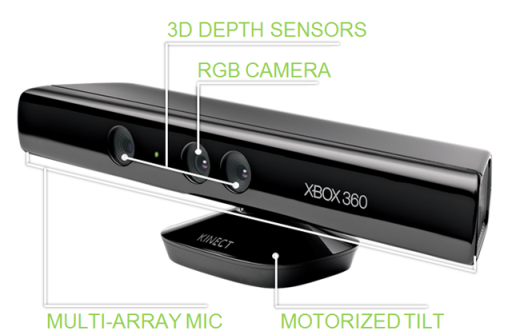
\includegraphics[scale=0.4]{image1}
\caption{The Microsoft Kinect is an example of a hybrid sensor called an RGBD camera. It captures 2D pixel arrays in 3 colour channels, in addition to capturing depth information using structured infra-red light pattern.}
\end{figure}

This project explores the perception of an environment using a hybrid sensor called an RGBD camera. This type of sensor captures a 2D pixel array on red, green, and blue channels using a monocular camera. Further, the sensor captures depth information by measuring the deformation of reflections from structured infra-red (IR) light emitted into the environment. The sensor will be employed using a WillowGarage PR2 robot simulated using ROS, Gazebo, and Rviz. A real world image of the PR2 can be seen in Figure 2, and a close up of the robot's sensing hardware can be seen in Figure 3.

\begin{figure}[H]
\centering
\begin{minipage}[t]{0.45\linewidth}
\centering
\frame{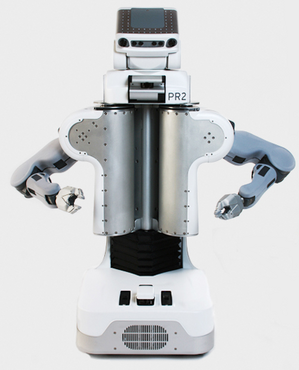
\includegraphics[height=4cm]{image2}}
\caption{A picture of the WillowGarage PR2 robot.}
\end{minipage}
\hspace{0.5cm}
\begin{minipage}[t]{0.45\linewidth}
\centering
\frame{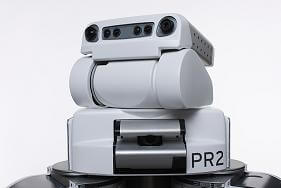
\includegraphics[height=4cm]{image3}}
\caption{A close up of the PR2's RGBD camera which captures image and depth data, and is used to create point clouds.}
\end{minipage}
\end{figure}

\begin{table}[h]
\centering
\caption{Examples of passive and active sensors which can be used for robotic perception systems (note that this list is not exhaustive)}
\begin{tabular}{p{2.3cm}p{4.5cm}p{2.3cm}p{4.5cm}}
\toprule
\multicolumn{2}{c}{\textbf{Passive Sensors}} & \multicolumn{2}{c}{\textbf{Active Sensors}}\\
\cmidrule(lr){1-2} \cmidrule(lr){3-4}
\textbf{Name} & \textbf{Description} & \textbf{Name} & \textbf{Description}\\
\midrule
Monocular Camera & A single RGB camera providing information on texture and shape & LIDAR & A 3D laser scanner which determines information about an environment through reading pulsed laser emission reflections\\
& & & \\
Stereo Camera & Consists of 2 monocular cameras providing the same information as the single monocular camera, but with the addition of depth information too & Time of Flight Camera & A 3D ToF camera performs depth measurement by illuminating environment with infra-red and observing the time taken to reflect from surfaces to the camera\\
& & & \\
& & Ultrasonic & Provides depth information by sending out high-frequency sound pulses and measuring time taken for sound to reverberate\\
\bottomrule
\end{tabular}
\end{table}

The captured sensor information is processed into a point cloud using the \verb|pcl| library which is implemented in ROS. Perception of an environment is not simply the capture of point cloud data, rather, it is the implementation of software in order to make sense of the point cloud data. The ultimate goal of this project is for the PR2 to identify objects on a table, pick these objects in a specified order, and stow them into the desired container either on the left or the right of the robot. In order to complete this task, there are two main sub-tasks that the robot's perception architecture must achieve: Segmentation, and Object Recognition. Segmentation is a complex process made up of many subtasks. Briefly, the segmentation implementation for this project is made up of the following sequence of activities:
\begin{enumerate}
\item Statistical filtering;
\item Voxel downsampling;
\item RANSAC plane filtering;
\item Passthrough filtering; and
\item Euclidean clustering (DBSCAN)
\end{enumerate}

These activities are applied to the captured point cloud data, and will be explored in more detail in Section 2. Object recognition is a similarly complex activity, which employs the uses of machine learning. There are numerous machine learning schemes that may be implemented in this instance, to varying degrees of effectiveness and computational cost. Irrespective of which machine learning algorithm is used, features which will be important to the developed model will need to be selected, and data captured which is used to train the model. This project employs the use of a supervised learning algorithm called a support vector machine and will be explored in more detail in Section 3.\\

The principal outcome from implementation of the segmentation and object recognition pipelines is to correctly classify objects on a table in front of the robot in a simulated environment. The objects will be household items varying in nature. The robot will need to segment the point cloud data into distinct clusters of points, and correctly classify each cluster of points. Success has been classified as receiving 100\% accuracy in test world one containing three objects; 80\% accuracy in test world two containing five objects; and 75\% accuracy in test world three containing eight objects.

\newpage

%--------------------------------------------------------------------------

\section{Segmentation}
\subsection{Statistical Filtering to Remove Image Noise}
As previously mentioned, the point cloud is obtained using an RGBD camera to capture a 2D image which consists of three feature maps, and a depth representation. The three feature maps represent the individual Red, Green, and Blue (RBG) channels for colour image. Each discrete pixel in the 2D array is also assigned an image depth. There are a total of 4 dimensions for each individual point in the point cloud which is assembled in the ROS environment by the \verb|pcl| library. The captured point cloud is not a perfect representation of the environment, rather, there are elements of noise introduced through dust, humidity, and light sources in the environment. Further, often instrumentation and transmission channels are imperfect which produce noise in the signal. The noisy signal can be seen in Figure 4 - the noise are the stochastic particles throughout the image. To remove the noise, a statistical outlier filter is used. This employs a Gaussian method to remove statistical outlier from the pointcloud. The implementation in the \verb|pcl_callback| function can be seen in Listing 1. A signal which has had noise removed can be seen in Figure 5. The successful implementation of the object recognition relies on clean segmentation of objects in a frame. The presence of noise results in the confusion of the Euclidean clustering method which provides segmentation, so it is important to apply this statistical filter prior to any further processing.

\vspace{1cm}

\begin{figure}[h]\scriptsize
\begin{sexylisting}{Obtain the point cloud and statistically filter to remove noise}
##############################################################################
    # Convert ROS msg to PCL data
##############################################################################
    cloud = ros_to_pcl(pcl_msg)

##############################################################################
    # Statistical Outlier Filtering
##############################################################################
    outlier_filter = cloud.make_statistical_outlier_filter()
    outlier_filter.set_mean_k(2)
    outlier_filter.set_std_dev_mul_thresh(0.5)
    cloud_filtered = outlier_filter.filter()
\end{sexylisting}
\end{figure}

\vspace{1cm}

\begin{figure}[h]
\centering
\begin{minipage}{0.45\linewidth}
\centering
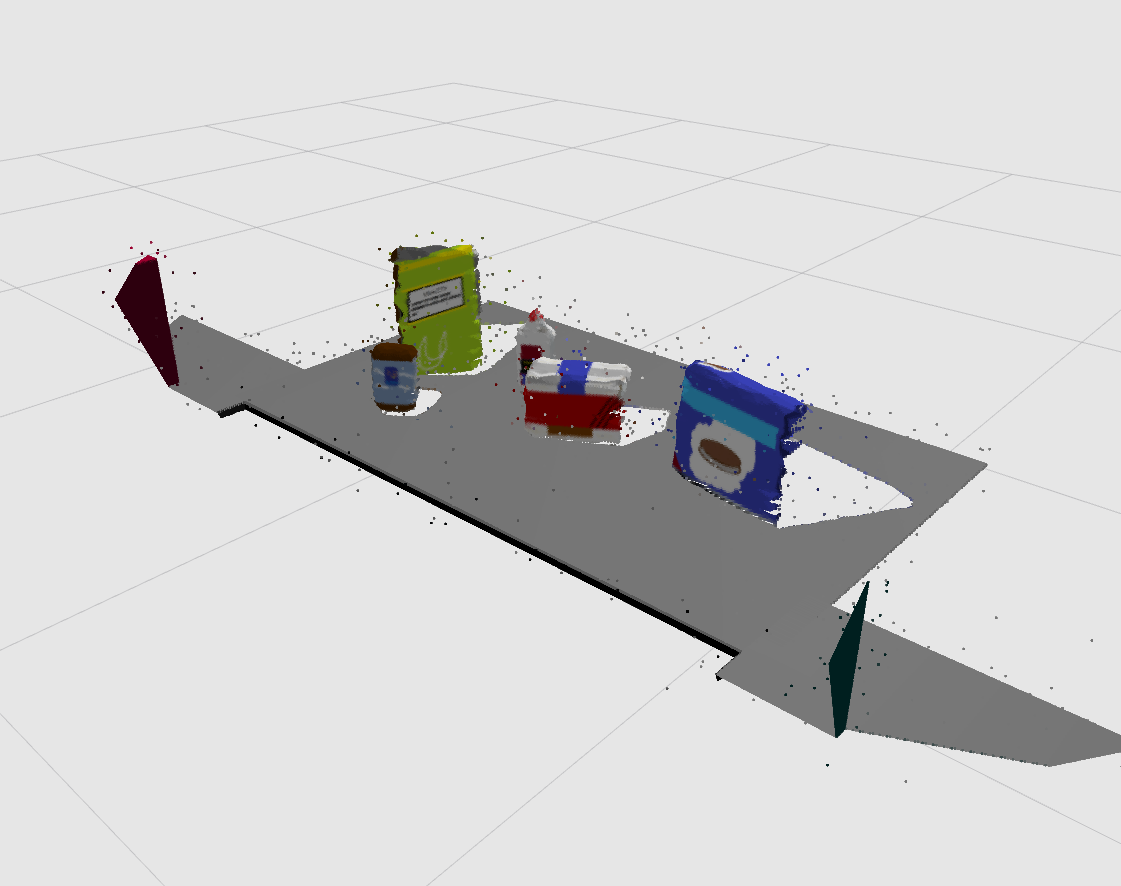
\includegraphics[scale=0.2]{image11}
\caption{Noisey point cloud of table and objects}
\end{minipage}
\hspace{0.5cm}
\begin{minipage}{0.45\linewidth}
\centering
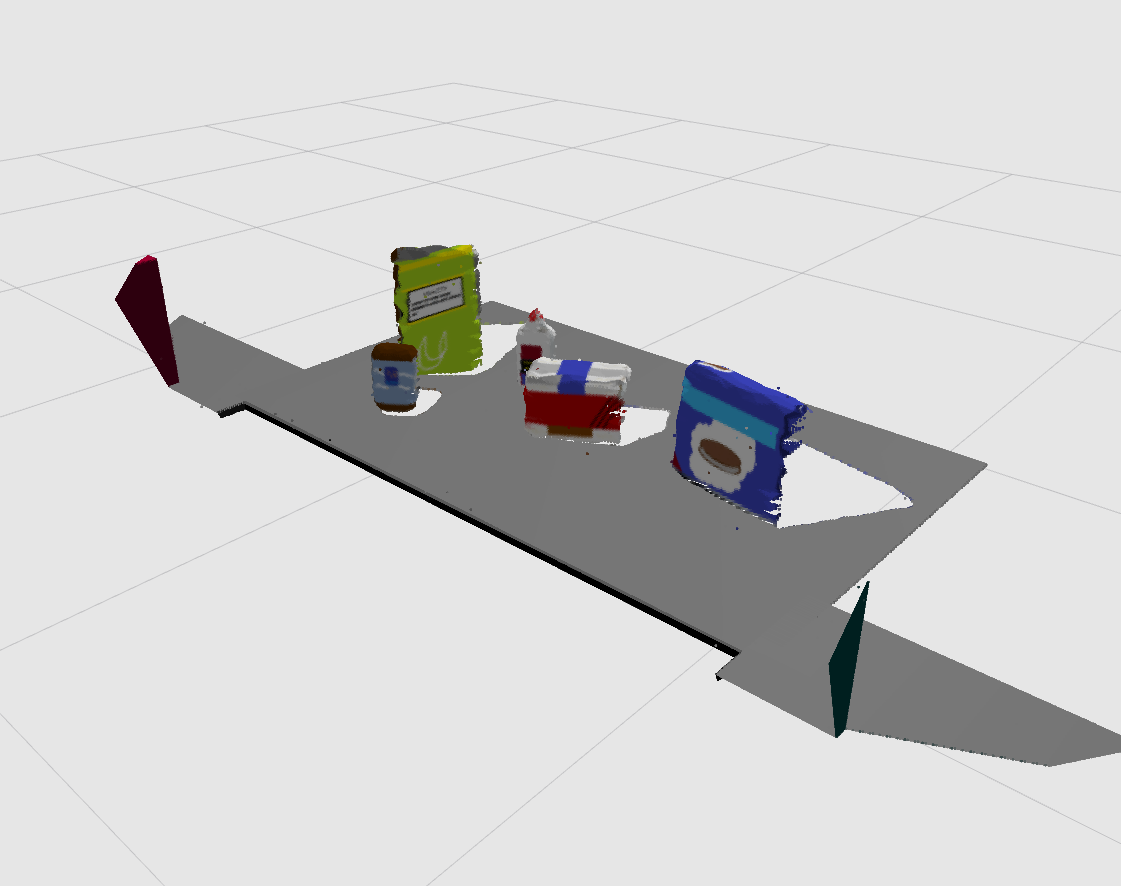
\includegraphics[scale=0.2]{image5}
\caption{The application of the Gaussian filter removes noise from the signal}
\end{minipage}
\end{figure}

\newpage

\subsection{Voxel Downsampling}
Point clouds often provide more data than necessary to achieve an accurate representation of the physical environment. The processing of this data, left unchecked, is computationally expensive. Downsampling is the process of removing data points in a systematic fashion, and is a technique that is often employed in the field of image processing. Voxel downsampling is analogous to the 2D process, that is, points in the three dimensional point cloud model are removed in a systematic fashion. Care needs to be taken when adjusting the parameters for the Voxel downsampling - if the downsampling is too aggressive, too much information may be removed compromising the ability to provide effective segmentation. The implementation of the Voxel downsampling can be seen in Listing 2. Figure 6 shows the pointcloud before Voxel downsampling, and Figure 7 shows the pointcloud after downsampling.

\vspace{1cm}

\begin{figure}[h]\scriptsize
\begin{sexylisting}{Obtain the point cloud}
##############################################################################
    # Voxel Grid Downsampling
##############################################################################
    # Create a VoxelGrid filter object for our input point cloud
    vox = cloud_filtered.make_voxel_grid_filter()

    # Choose a voxel (also known as leaf) size
    LEAF_SIZE = 0.01

    # Set the voxel (or leaf) size
    vox.set_leaf_size(LEAF_SIZE, LEAF_SIZE, LEAF_SIZE)

    # Call the filter function to obtain the resultant downsampled point cloud
    cloud_filtered = vox.filter()
\end{sexylisting}
\end{figure}

\vspace{1cm}

\begin{figure}[h]
\centering
\begin{minipage}{0.45\linewidth}
\centering
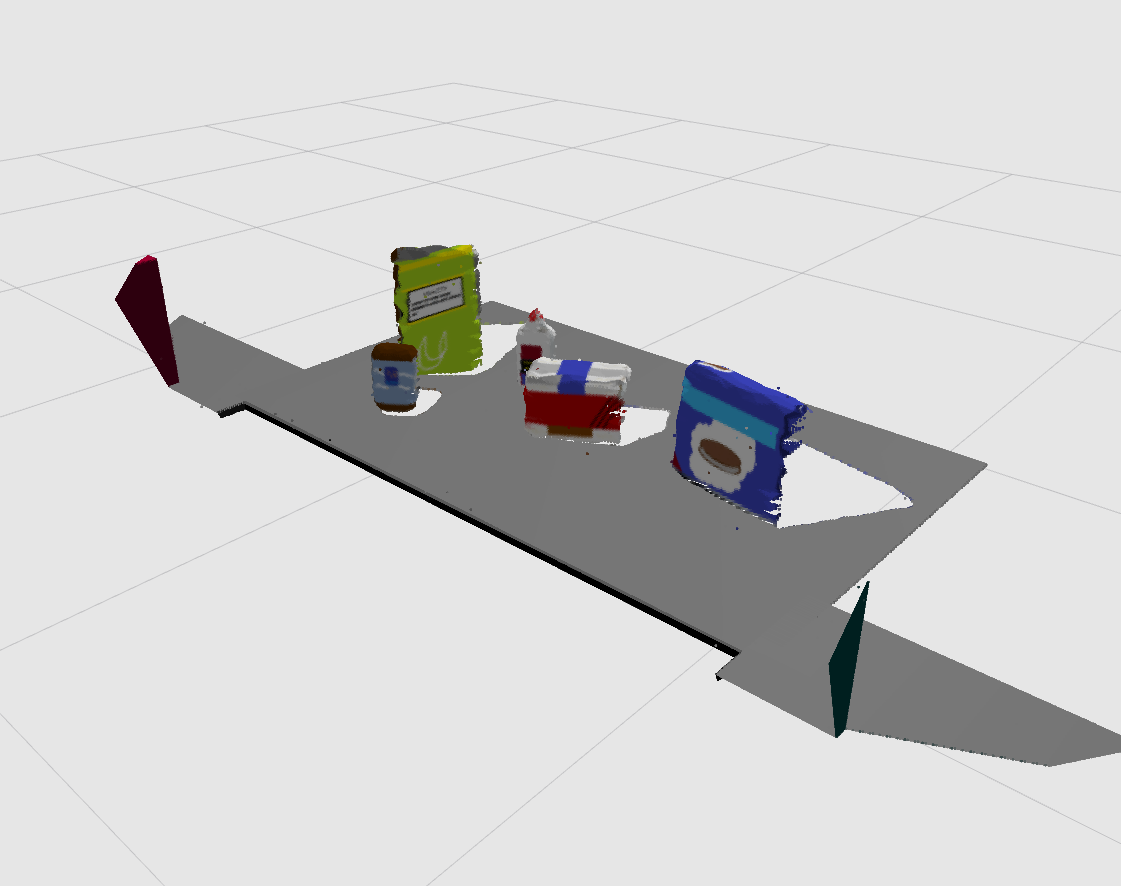
\includegraphics[scale=0.2]{image5}
\caption{include a figure which shows no Voxel Downsampling}
\end{minipage}
\hspace{0.5cm}
\begin{minipage}{0.45\linewidth}
\centering
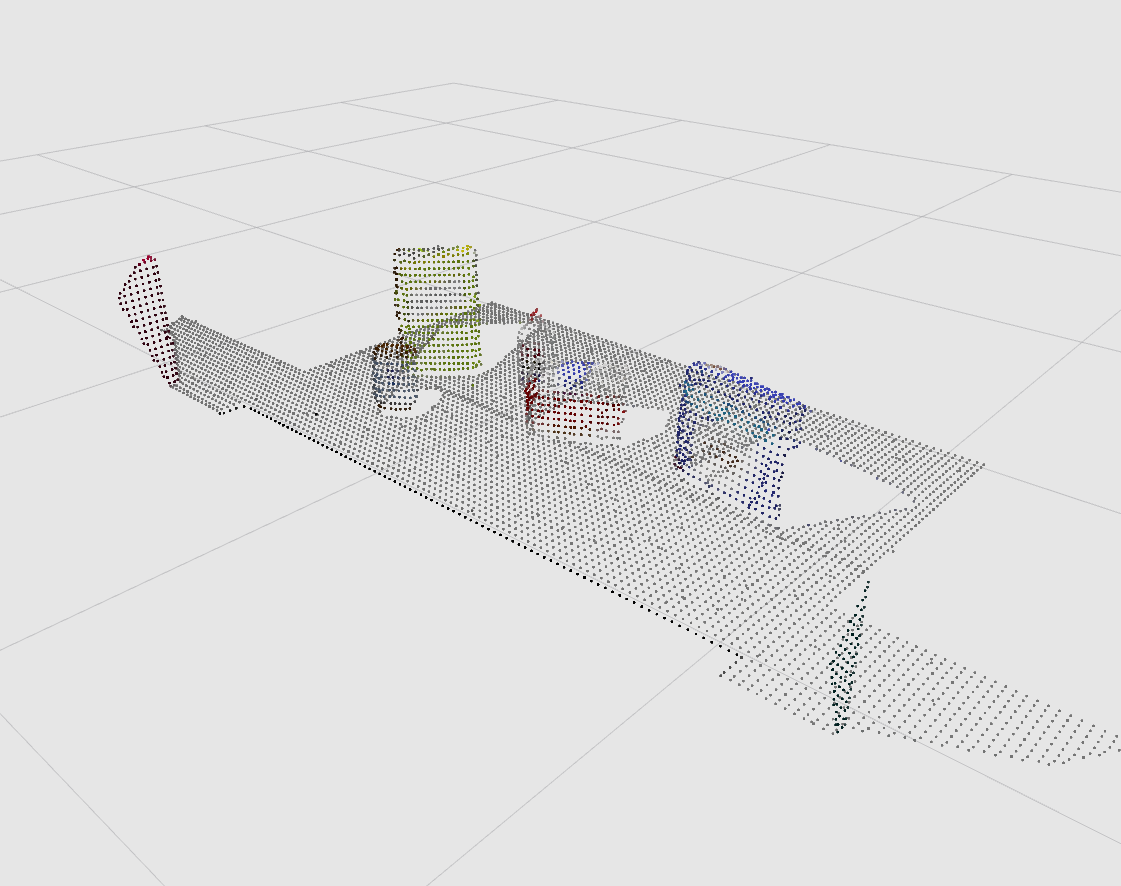
\includegraphics[scale=0.2]{image10}
\caption{include a figure which shows the basics of Voxel Downsampling}
\end{minipage}
\end{figure}

\newpage

\subsection{Passthrough Filtering}
A pass through filter is a simply designed to remove points from the point cloud which fall outside a spatially bounded region. This filter is very basic in its implementation, and does not rely on any statistical filters to achieve the results. The implementation can be seen in Listing 4. In this instance, we remove points which don't fall within an area bounded by a rectangular prism. Whilst this filtering is not essential, it helps stops the robot from segmenting points which belong to the boxes which lie to the left and right of the robot's work space. It also removes the robot's arms from the point cloud. Figure 8 shows the unfiltered pointcloud, and Figure 9 shows the pointcloud after the passthrough filter has been applied.

\vspace{1cm}

\begin{figure}[h]\scriptsize
\begin{sexylisting}{Obtain the point cloud}
##############################################################################
    # PassThrough Filter
##############################################################################
    # Create a PassThrough filter object.
    passthrough_z = cloud_filtered.make_passthrough_filter()

    # ZAXIS Assign axis and range to the passthrough filter object.
    filter_axis = 'z'
    passthrough_z.set_filter_field_name(filter_axis)
    axis_min = 0.60
    axis_max = 1.8
    passthrough_z.set_filter_limits(axis_min, axis_max)

    # Use the filter function to obtain the filtered z-axis.
    cloud_filtered = passthrough_z.filter()

    # Create PassThrough filter object
    passthrough_y = cloud_filtered.make_passthrough_filter()

    # YAXIS Assign axis and range to the passthrough filter object
    filter_axis = 'y'
    passthrough_y.set_filter_field_name(filter_axis)
    axis_min = -0.5
    axis_max = 0.5
    passthrough_y.set_filter_limits(axis_min, axis_max)

    # Use the filter function to obtain the filtered y-axis
    cloud_filtered = passthrough_y.filter()
\end{sexylisting}
\end{figure}

\vspace{1cm}

\begin{figure}[h]
\centering
\begin{minipage}{0.45\linewidth}
\centering
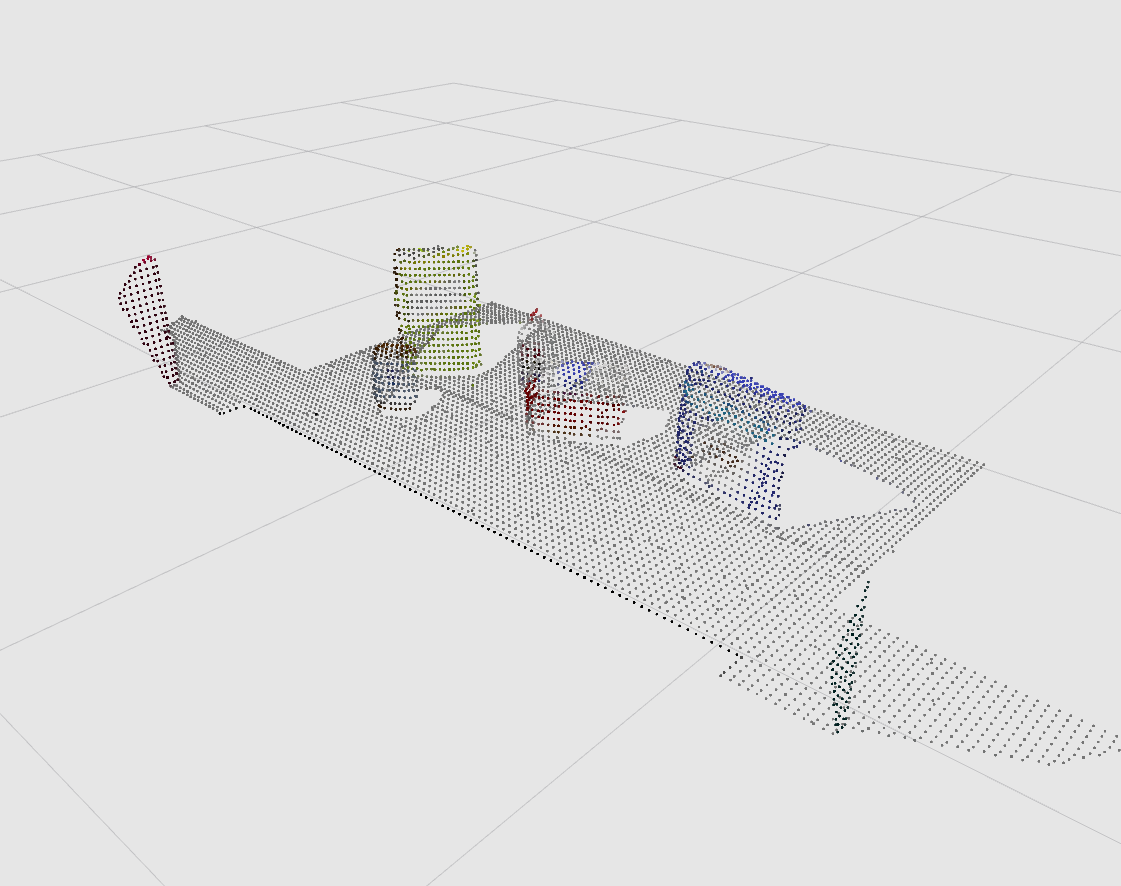
\includegraphics[scale=0.2]{image10}
\caption{Include and image of the unfiltered point cloud}
\end{minipage}
\hspace{0.5cm}
\begin{minipage}{0.45\linewidth}
\centering
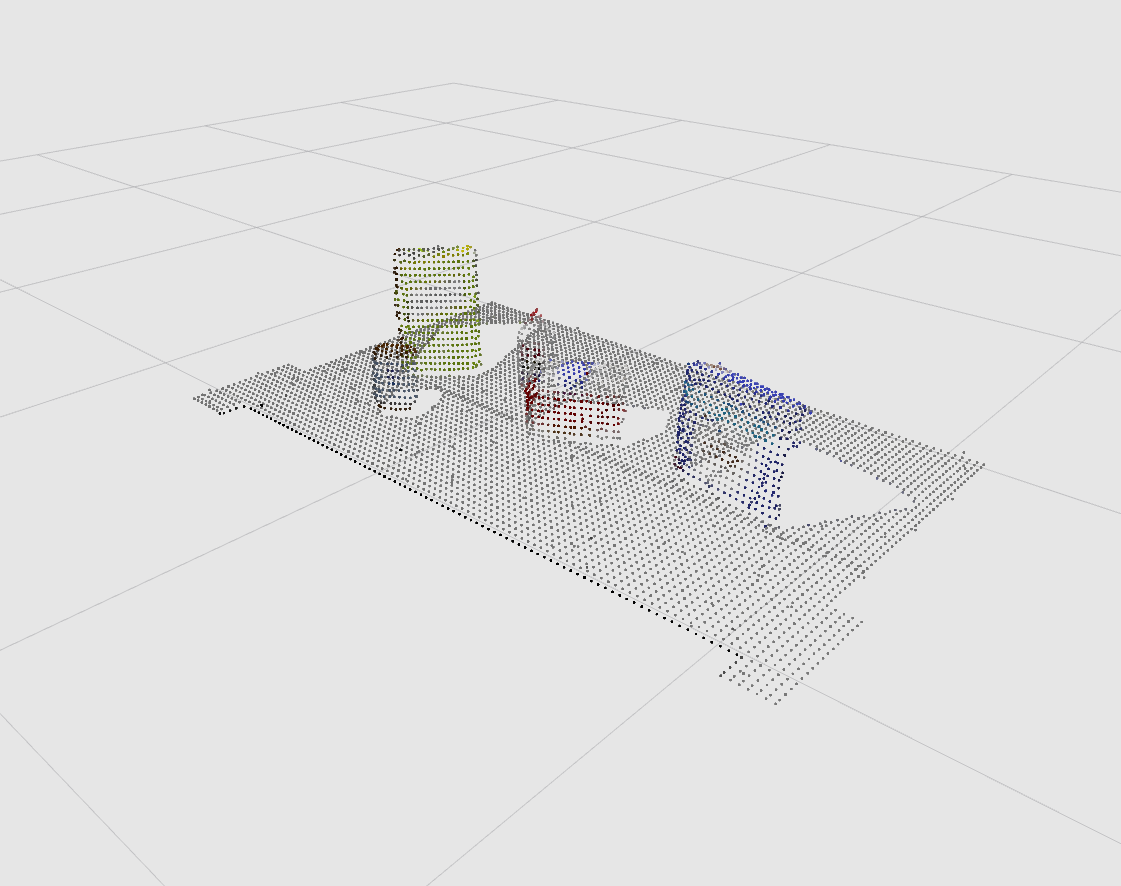
\includegraphics[scale=0.2]{image7}
\caption{Include an image of the filtered point cloud}
\end{minipage}
\end{figure}

\newpage

\subsection{RANSAC Plane Segmentation}
Random sample consensus (RANSAC) is an segmentation algorithm which detects statistical outliers which do not fit a geometrical mathematical model. The mathematical model is specified depending on the filtering requirement. In this instance the mathematical model being used is a plane, which closely resembles the table which the objects sit on in the point cloud image. The model outliers, that is those points which don't statistically fit the mathematical representation of a plane, are filtered from the point cloud. Filtered points which fit the model are stored in the variable \verb|could_table|, and those that don't fit the model are stored in the variable \verb|cloud_objects|. This processing helps to isolate the objects in the image, ready for segmentation and object recognition. The implementation can be seen in Listing 4. The filtered could points which fit the model can be seen in Figure 10 - the table has been extracted. The remaining points, the outliers, can be seen in Figure 11. Including the table in the pointcloud image creates a potential opportunity to confuse the Euclidean clustering algorithm since the segmentation is based on spatial proximity. Further benefits include the decreased computation cost for processing the remainder of the point cloud.

\vspace{0.25cm}

\begin{figure}[h]\scriptsize
\begin{sexylisting}{Obtain the point cloud}
##############################################################################
    # RANSAC Plane Segmentation
##############################################################################
    # Create the segmentation object
    seg = cloud_filtered.make_segmenter()

    # Set the model you wish to fit
    seg.set_model_type(pcl.SACMODEL_PLANE)
    seg.set_method_type(pcl.SAC_RANSAC)

    # Max distance for a point to be considered fitting the model
    max_distance = 0.01
    seg.set_distance_threshold(max_distance)

    # Call the segment function to obtain set of inlier indices and model coefficients
    inliers, coefficients = seg.segment()
    
##############################################################################
    # Extract inliers and outliers
##############################################################################
    # Extract inliers
    cloud_table = cloud_filtered.extract(inliers, negative=False)

    # Extract outliers
    cloud_objects = cloud_filtered.extract(inliers, negative=True)
\end{sexylisting}
\end{figure}

\vspace{0.25cm}

\begin{figure}[h]
\centering
\begin{minipage}{0.45\linewidth}
\centering
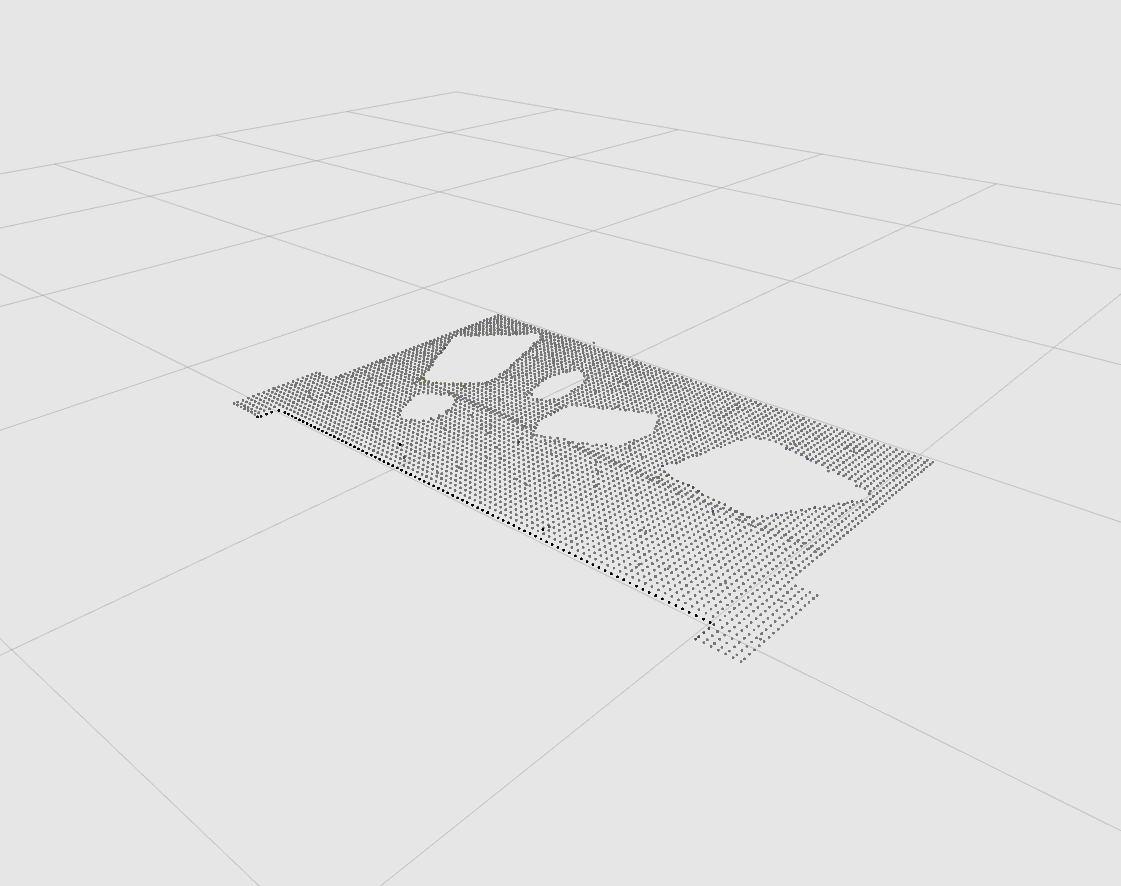
\includegraphics[scale=0.2]{image6}
\caption{Include an image of filtered point cloud table}
\end{minipage}
\hspace{0.5cm}
\begin{minipage}{0.45\linewidth}
\centering
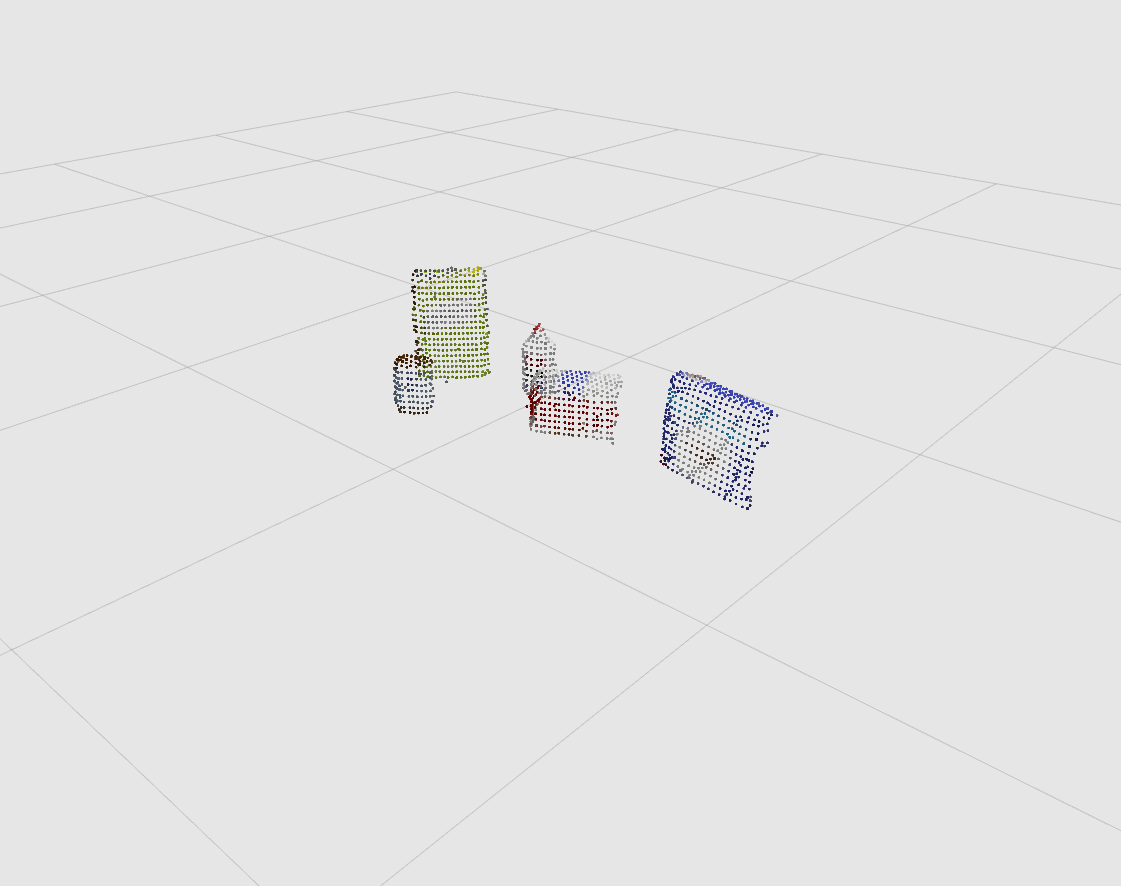
\includegraphics[scale=0.2]{image8}
\caption{Include an image of the filtered point cloud which has all of the objects only}
\end{minipage}
\end{figure}

\newpage

\subsection{Euclidean Clustering (DBSCAN)}
Segmentation is undertaken using a Euclidean clustering algorithm called DBSCAN - the implementation can be seen in Listing 5. The algorithm is a density based spatial clustering algorithm. Typically this algorithm is employed when k-means clustering is not appropriate, that is,  points in the point cloud together based on their proximity to each other.

Potential problems with this method. This method encounters problems if the objects are too close to each other. If the objects are too close to each other, then the Euclidean clustering method fails - the algorithm will think that the objects 

\vspace{0.5cm}

\begin{figure}[h]\scriptsize
\begin{sexylisting}{Apply Euclidean clustering to the pointcloud}
##############################################################################
    # Extract inliers and outliers
##############################################################################
    # Extract inliers
    cloud_table = cloud_filtered.extract(inliers, negative=False)

    # Extract outliers
    cloud_objects = cloud_filtered.extract(inliers, negative=True)


##############################################################################
    # Euclidean Clustering
##############################################################################
    white_cloud = XYZRGB_to_XYZ(cloud_objects)
    tree = white_cloud.make_kdtree()

    # Create a cluster extraction object
    ec = white_cloud.make_EuclideanClusterExtraction()

    # Set tolerances for distance threshold
    # as well as minimum and maximum cluster size (in points)
    ec.set_ClusterTolerance(0.05)
    ec.set_MinClusterSize(50)
    ec.set_MaxClusterSize(3000)

    # Search the k-d tree for clusters
    ec.set_SearchMethod(tree)

    # Extract indices for each of the discovered clusters
    cluster_indices = ec.Extract()
\end{sexylisting}
\end{figure}

\vspace{0.5cm}

\begin{figure}[h]
\centering
\begin{minipage}{0.45\linewidth}
\centering
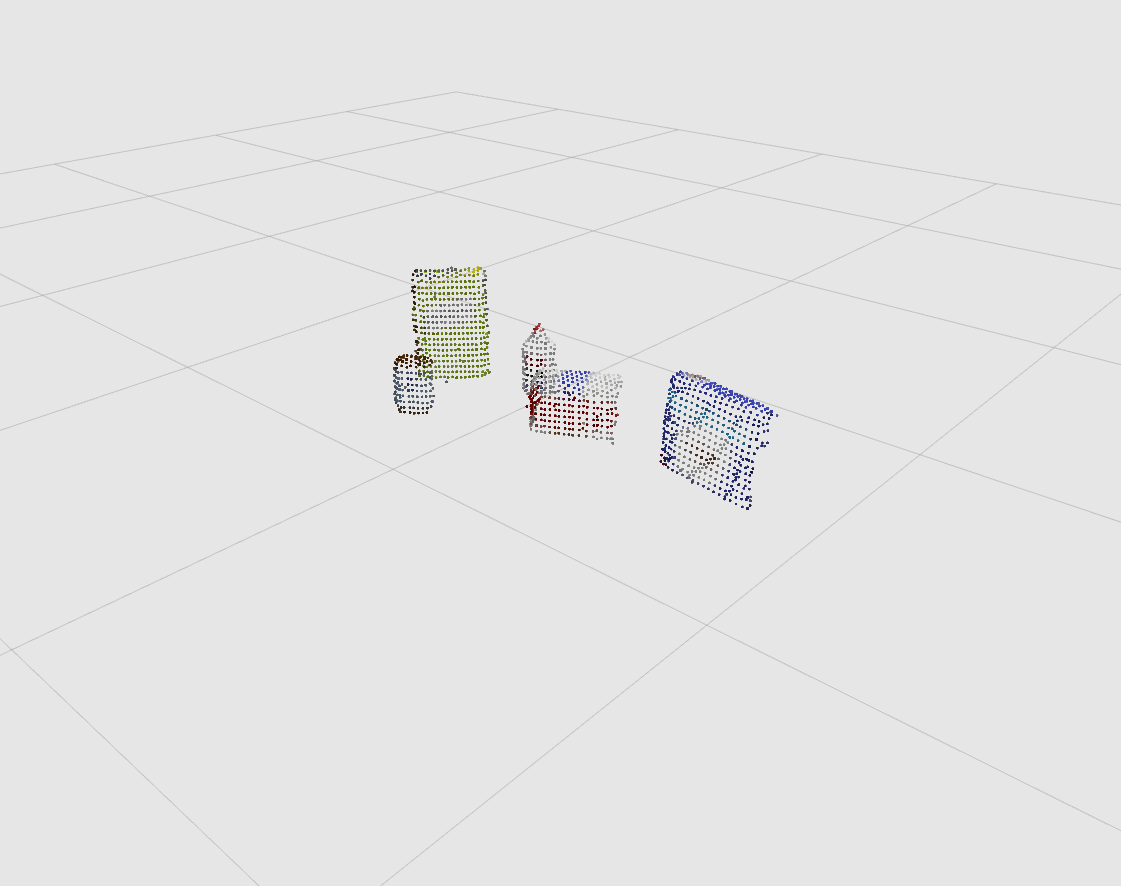
\includegraphics[scale=0.2]{image8}
\caption{Include and image of the unfiltered point cloud}
\end{minipage}
\hspace{0.5cm}
\begin{minipage}{0.45\linewidth}
\centering
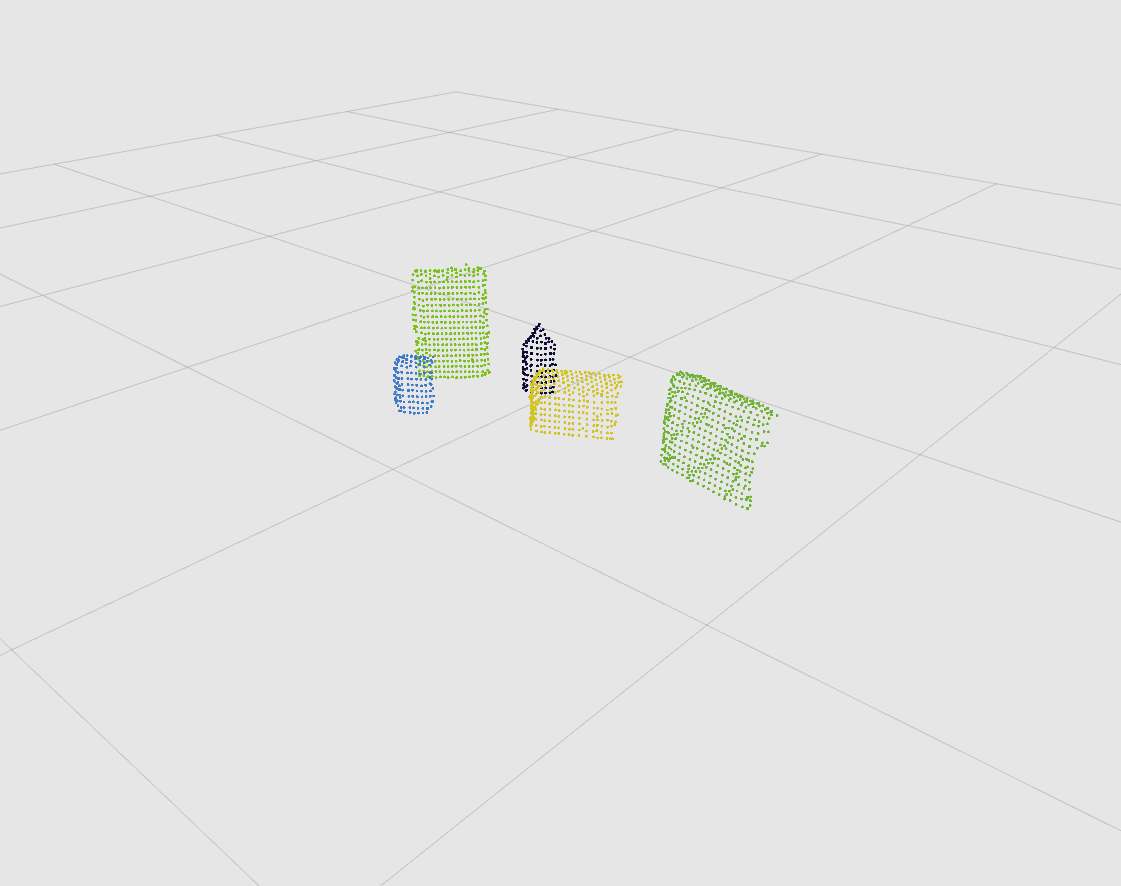
\includegraphics[scale=0.2]{image9}
\caption{Include an image of the filtered point cloud}
\end{minipage}
\end{figure}

\begin{figure}[h]\scriptsize
\begin{sexylisting}{Assign a mask colour to each segment of the segmented point cloud}
##############################################################################
    # Create Cluster-Mask Point Cloud to visualize each cluster separately
##############################################################################
    #Assign a color corresponding to each segmented object in scene
    cluster_color = get_color_list(len(cluster_indices))

    color_cluster_point_list = []

    for j, indices in enumerate(cluster_indices):
        for i, indice in enumerate(indices):
            color_cluster_point_list.append([white_cloud[indice][0],
                                            white_cloud[indice][1],
                                            white_cloud[indice][2],
                                            rgb_to_float(cluster_color[j])])

    #Create new cloud containing all clusters, each with unique color
    cluster_cloud = pcl.PointCloud_PointXYZRGB()
    cluster_cloud.from_list(color_cluster_point_list)
\end{sexylisting}
\end{figure}


\section{Object Recognition}
Object recognition allows a robot to correctly locate an object of interest in the environment. The first step in this process is to distinguish between point cloud data which belong to objects, from point cloud data belonging to the environment. This has been achieved using Passthrough filtering, and RANSAC plane segmentation. Following this, the set of point cloud data points belonging to an individual object need to be identified - this has been achieved using Euclidean Clustering (DBSCAN). Once these two steps are correctly implemented, the task of identifying an object can be simplified to identifying a set of features in the object point cloud data which  match the object of interest.\\

The robot is required to distinguish between different household items, with each scene containing no more than eight objects at a time. The objects are laid out on the table in front of the robot in randomised configurations. A typical set of objects placed in a scene is shown in Figure 14.
\begin{figure}[h]
\centering
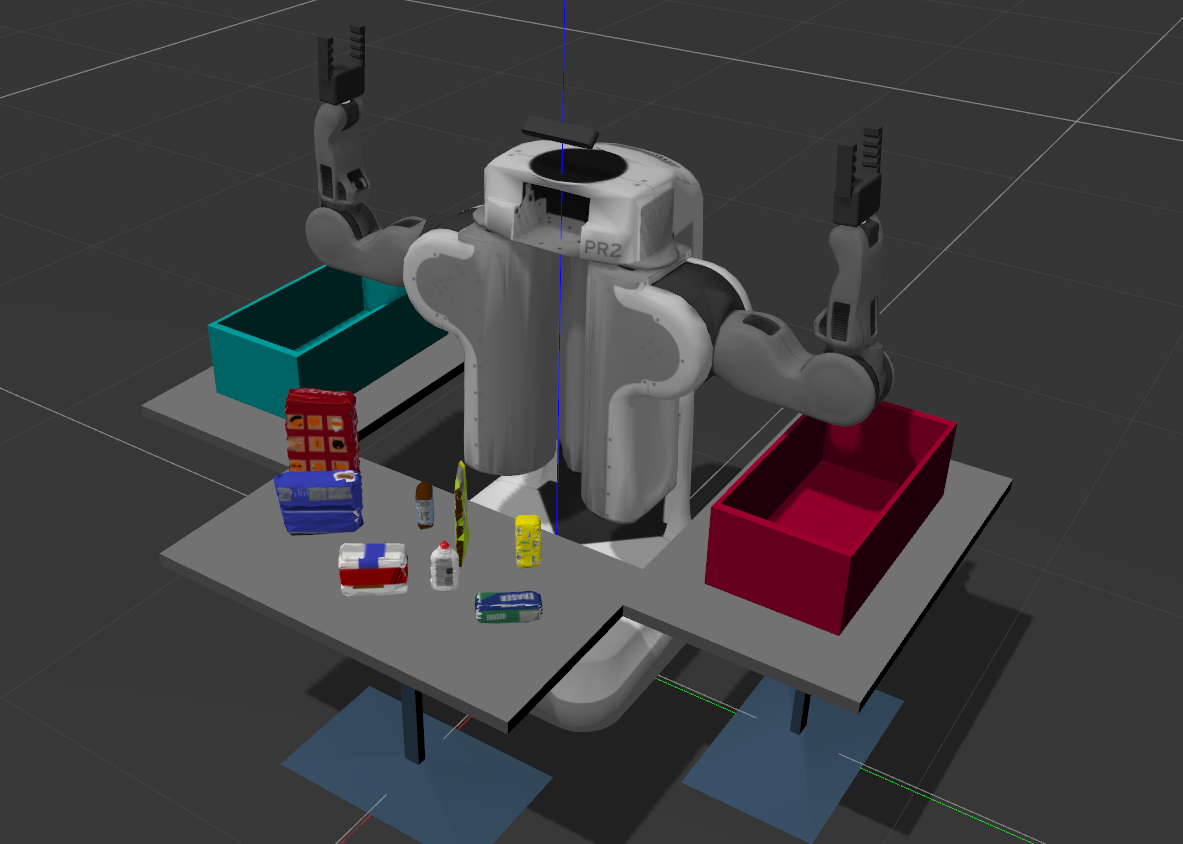
\includegraphics[scale=0.15]{object_layout}
\caption{An example of a typical object layout scenario. The PR2 robot can be seen with its arms raised, and the objects are laid out on the table in front of it.}
\end{figure}

This project sees the implementation of a machine learning application as the main instrument the robot will use to distinguish between objects. There are many competing models that could be used, but a supervised learning model called a Support Vector Machine (SVM) has been chosen for ease of implementation and a demonstrated reliability in simple tasks like this one. It is not the intention of this paper to discuss the mathematical underpinnings of SVM, however, the central mechanism for classification is achieved by fitting hyperplanes to the feature space such that there is a maximum `boundry' between the data and the hyperplanes for each object region.
\newpage
\subsection{Object Features}
\begin{minipage}{0.66\textwidth}
The object shown in Figure 15 has two useful data sets that we can expoit for a machine learning application: colour, and object shape. Capturing colour data requires an understanding of how colour is represented digitally. There are many choices for representing colour spaces, however, normally either Red, Green, and Blue (RGB), or Hue, Saturation, and Value (HSV) are chosen for computer vision applications. The main reason for these choices are due to a well established code base for RGB and HSV. Also there are many packages providing conversion between the two, making for easy implementation. RGB and HSV colour spaces are shown in Figures 16 and 17, respectively. Which colour space is best for this application? Both would suffice, however, there is an advantage of choosing HSV. The HSV colour space separates the \textit{luma} (colour intensity), from the \textit{chroma} (colour information). This is desirable because it makes colour data less susceptible to changes in lighting, or shadows, resulting in more robust performance from machine learning models.
\end{minipage}
\hspace{0.5cm}
\begin{minipage}{0.33\textwidth}
		\centering
		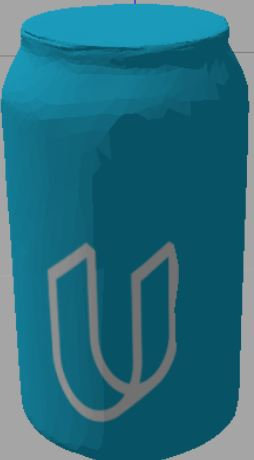
\includegraphics[scale=0.5]{can_image}
		\captionof{figure}{An example of a simulated object.}
\end{minipage}
	
\vspace{0.5cm}
 
\begin{figure}[h]
	\centering
	\begin{minipage}{0.45\textwidth}
		\centering
		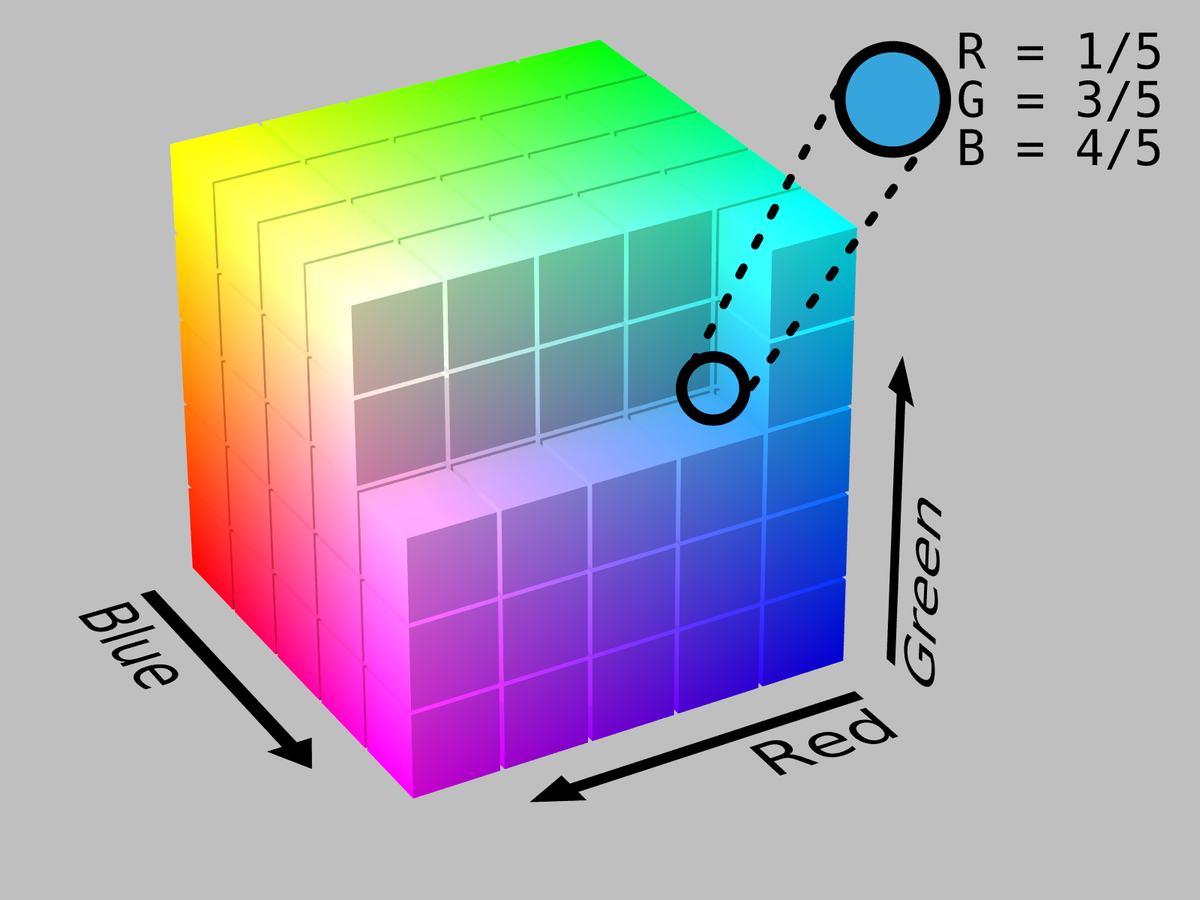
\includegraphics[height=5cm]{RGB_colour_space}
		\caption{Red, Green, and Blue colour space.}
	\end{minipage}
	\hspace{1cm}
	\begin{minipage}{0.45\textwidth}
		\centering
		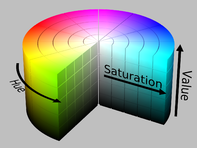
\includegraphics[height=5cm]{HSV_colour_space}
		\caption{Hue, Saturation, and Value colour space.}
	\end{minipage}
\end{figure}

Shape based data allows for the description of the object surface. Whilst there are many mathematical descriptions for manifold surfaces which we may employ, a simple idea to capture this information uses surface normals discretely distributed over the object surface.

\begin{minipage}{0.45\textwidth}
Figure 18 shows a surface with a series of normal vectors located at discrete points over the surface as described. Finally, deciding on the type data to capture is only one part of the problem when considering model features. Once we have the data, how should it be represented. One effective way used in computer vision applications is to build histograms of the HSV colours and surface normals profiles to obtain an estimate of the distributio. Section 3.2 and Section 3.3 discuss the process of using histograms to create features in more detail.
\end{minipage}
	\hspace{1cm}
\begin{minipage}{0.45\textwidth}
	\centering
	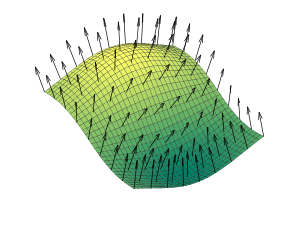
\includegraphics[height=5.5cm]{surface_normals}
	\captionof{figure}{Surface normals on a surface.}
\end{minipage}


\subsection{Colour Histograms}
Once the RGB image data has been captured from the RGBD camera, it is converted into HSV values for each pixel in the image. A histogram is then created for the HSV data using bin ranges from 0 to 256, with approximately 70 bins. An example of a continuous HSV histogram can be seen in Figure 19. The function implementation used to create colour histograms for the PR2 can be seen in Listing 7.
\begin{figure}[h]
	\centering
	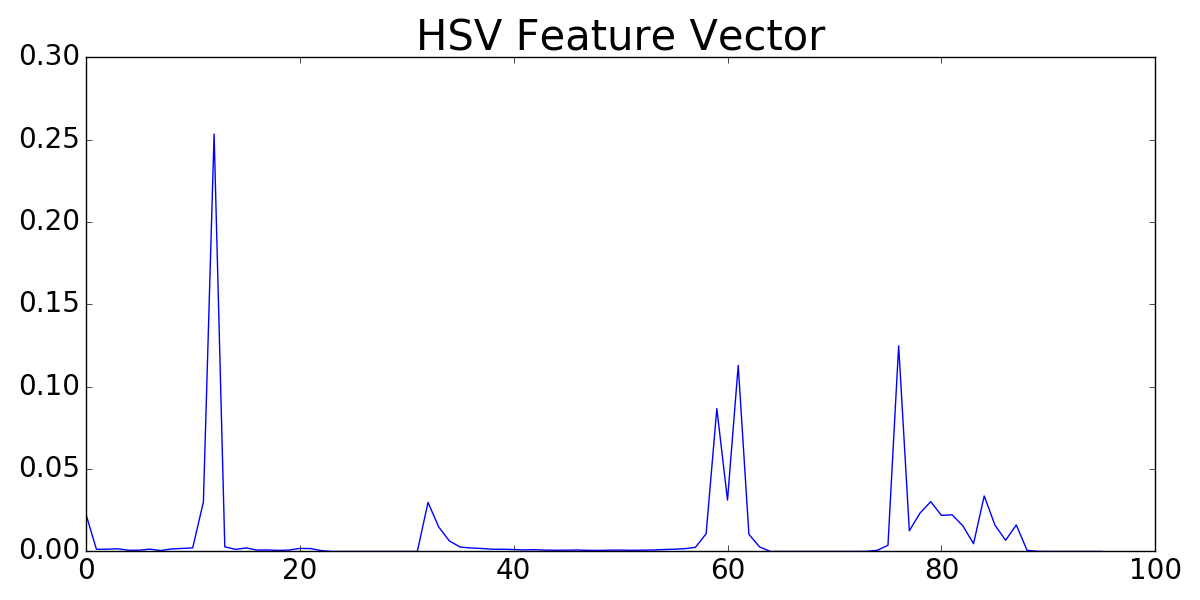
\includegraphics[height=4.5cm]{hsv_histo}
	\caption{A HSV histogram of the can object shown in Figure 15.}
\end{figure}

\begin{figure}[h]\scriptsize
\begin{sexylisting}{A function which returns a colour histogram for a point cloud}
def compute_color_histograms(cloud, using_hsv=False):

	# Compute histograms for the clusters
	point_colors_list = []

	# Step through each point in the point cloud
	for point in pc2.read_points(cloud, skip_nans=True):
		rgb_list = float_to_rgb(point[3])
		if using_hsv:
			point_colors_list.append(rgb_to_hsv(rgb_list) * 255)
		else:
			point_colors_list.append(rgb_list)

	# Populate lists with color values
	channel_1_vals = []
	channel_2_vals = []
	channel_3_vals = []

	for color in point_colors_list:
		channel_1_vals.append(color[0])
		channel_2_vals.append(color[1])
		channel_3_vals.append(color[2])

	# TODO: Compute histograms
	h_hist = np.histogram(channel_1_vals, bins=70, range=(0, 256))
	s_hist = np.histogram(channel_2_vals, bins=70, range=(0, 256))
	v_hist = np.histogram(channel_3_vals, bins=70, range=(0, 256))

	# TODO: Concatenate and normalize the histograms
	features = np.concatenate((h_hist[0], s_hist[0], v_hist[0])).astype(np.float64)
	# Generate random features for demo mode.
	# Replace normed_features with your feature vector
	normed_features = features/np.sum(features)

	return normed_features		
\end{sexylisting}
\end{figure}

\newpage

\subsection{Surface Normal Histograms}
Once the surface normal data has been captured a histogram is created using bin ranges from -1.1 to 1.1, given that the surface normals are confined to this range. The function implementation used to create surface normal histograms for the PR2 can be seen in Listing 8.
\begin{figure}[h]\scriptsize
\begin{sexylisting}{A function which returns a surface normal histogram for a given point cloud}
def compute_normal_histograms(normal_cloud):
	norm_x_vals = []
	norm_y_vals = []
	norm_z_vals = []

	for norm_component in pc2.read_points(normal_cloud,
	field_names = ('normal_x', 'normal_y', 'normal_z'),
	skip_nans=True):
		norm_x_vals.append(norm_component[0])
		norm_y_vals.append(norm_component[1])
		norm_z_vals.append(norm_component[2])

	# TODO: Compute histograms of normal values (just like with color)
	x_hist = np.histogram(norm_x_vals, bins=50, range=(-1.1,1.1))
	y_hist = np.histogram(norm_y_vals, bins=50, range=(-1.1,1.1))
	z_hist = np.histogram(norm_z_vals, bins=50, range=(-1.1,1.1))

	# TODO: Concatenate and normalize the histograms
	features = np.concatenate((x_hist[0], y_hist[0], z_hist[0])).astype(np.float64)
	# Generate random features for demo mode.
	# Replace normed_features with your feature vector
	normed_features = features/np.sum(features)

	return normed_features	
\end{sexylisting}
\end{figure}

\subsection{Capturing Data}
In order to generate enough meaningful data for our SVM classifier model, a script called\\ \verb|capture_feature.py| was implemented. This script, in conjunction with a ROS simulation of the RGBD camera, removes gravity so that a known object model floats in front of the RGBD sensor. The object is assigned randomised Roll, Pitch, and Yaw configurations for a set number of iterations. At each new orientation, the simulated RGBD sensor will capture point cloud data. From each of these point clouds we extract RGB, and surface normals to create histogram features. The object model label (e.g. biscuits) is saved, along with the HSV and surface normal histogram features. The full implementation of \verb|capture_features.py| can be found in Appendix A. Figure 20 shows an example of data being captured for an object model.
\begin{figure}[h]
	\centering
	\frame{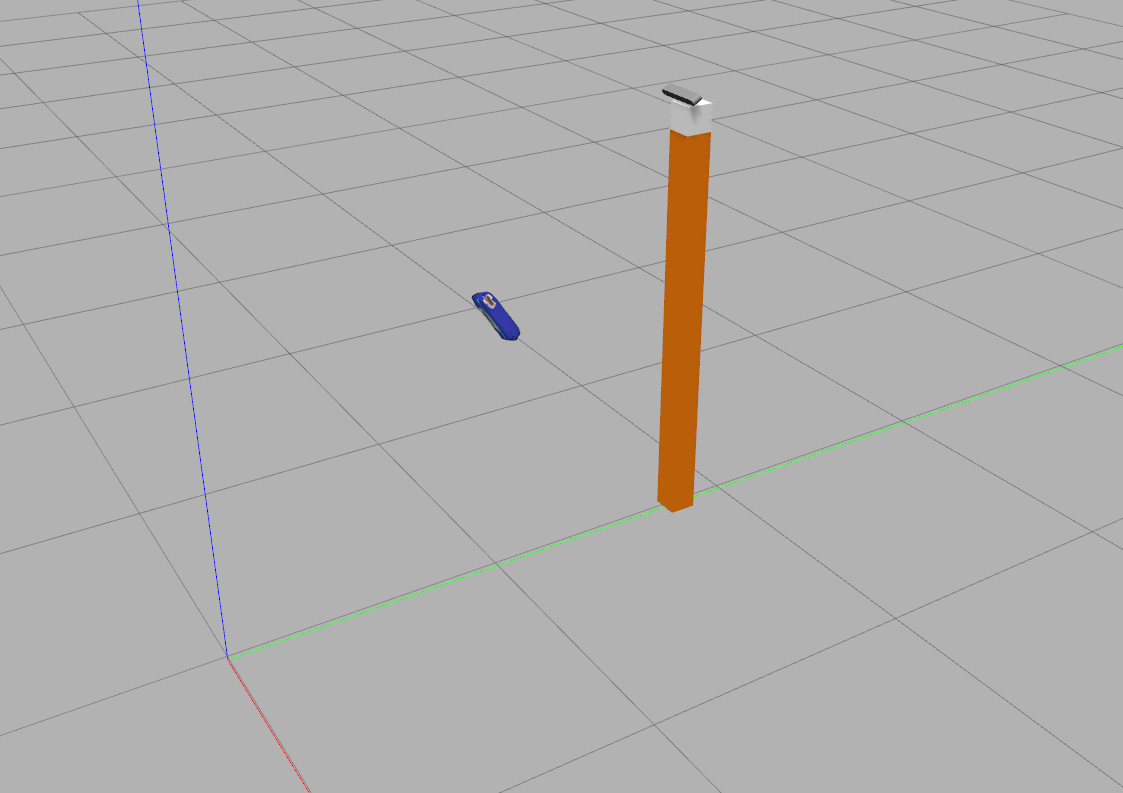
\includegraphics[scale=0.17]{capture_features}}
	\caption{The RGBD sensor is elevated in the world, placed on top of a stick. The object is flashed in at randomised orientations and point cloud data is captured.}
\end{figure}

\subsection{Training the SVM}
Once the dataset has been captured the Python library \verb|sklearn| was used to create a SVM classification model. This was implemented in a script called \verb|train_svm.py|, which can be seen in full in Appendix B. There are a couple of choices that can be made when optimising SVM performance. The first choice is between RGB or HSV colour spaces for our colour histogram feature (this choice is actually implemented in \verb|capture_features.py|, but discussion of this choice is more suited to this section). Table 2 shows reported model accuracy for two identical scenarios - the iterations was kept small at five, and the kernel for the SVM was linear, however,  one scenario used RGB and the other HSV. There is an observable performance increase to the SVM classifier when using HSV.
\begin{table}[h]
	\centering
	\caption{Accuracy of SVM using RGB and HSV colour spaces, holding other variables constant}
	\begin{tabular}{cccc}
		\toprule
		\textbf{Iterations} & \textbf{Colour Space} & \textbf{Kernel} & \textbf{Accuracy}\\
		\midrule
		5 & RGB & Linear & 57.5\%\\
		5 & HSV & Linear & 77.5\%\\
		\bottomrule
	\end{tabular}
\end{table}

The other choice to make is the kernel function that is used for the SVM. Python library \verb|sklearn| provides four off-the-shelf choices of kernel: linear, polynomial, rbf, and sigmoid. The best choice of kernel is not immediately clear. Figure 21 shows the performance of the four kernels for for an increasing number of iterations.  
\begin{figure}[h]
	\centering
	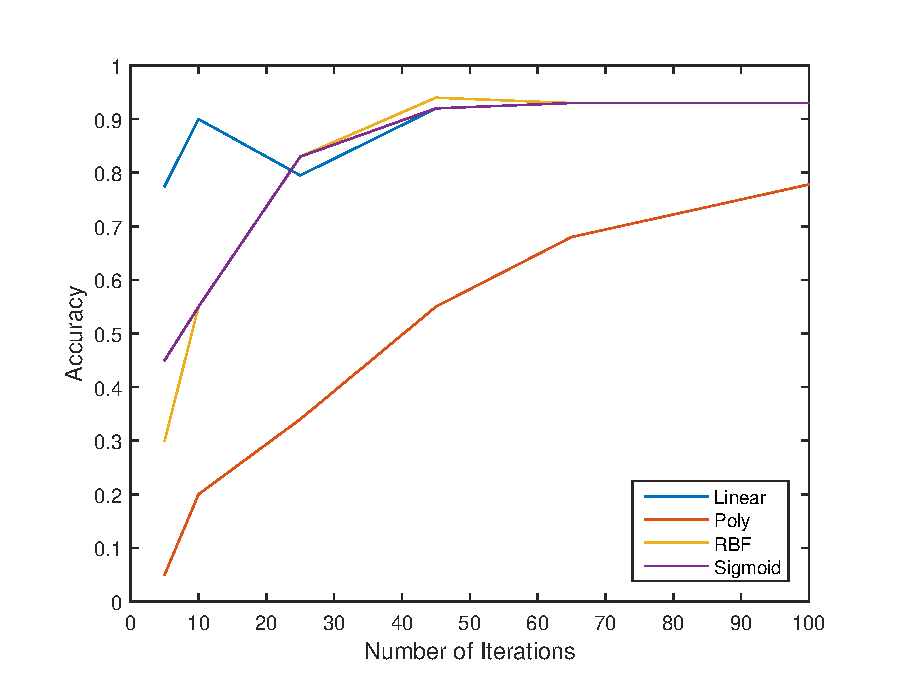
\includegraphics[scale=0.6]{kernels}
	\caption{The accuracy of each kernel for the SVM improves as the number of observations increases. Most kernels converge on 93\%.}
\end{figure}

At 100 iterations for each object, there is no immediate distinction between the linear, rbf, and sigmoid models - most likely due to overfitting. One avenue to improve the performance further would be the use of regularisation, however, this has not been used in this instance. Experimentation with the PR2 robot implementation of the sensor revealed that the sigmoid kernel provided the most reliable performance. The normalised confusion matrix for 100 iterations using the sigmoid kernel can be seen in Figure 22. Notably, the model finds it difficult to distinguish between the box of snack and the book.
\begin{figure}[h]
	\centering
	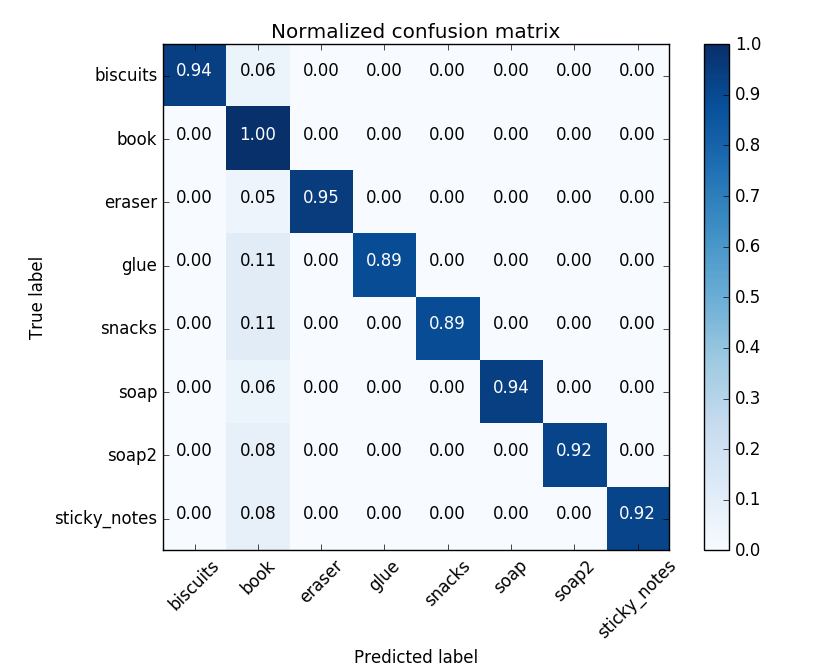
\includegraphics[scale=0.55]{normalised_confusion_matrix}
	\caption{Confusion matrix for the sigmoid kernal, with HSV colour space, and 100 observations per object. Figure shows the probabilities that a given object will be classified correctly. Additionally, the matrix shows what the probabilities are for misclassification.}
\end{figure}
\newpage

\section{PR2 Implementation \& YAML File Output}
The full implementation of the \verb|object detection.py| Python script, which is designed to be run in conjunction with a ROS simulation of the PR2 robot, can be found in Appendix C. The first part of the executed code initialises the publishers and subscribers, loads the perviously trained SVM model, and puts ROS into a persistant loop with \verb|rospy.spin()|. The ROS subscriber makes a call to the \verb|pcl_callback()| function everytime it receives point cloud data. This section of the code is shown  Listing 9. The initial part of the \verb|pcl_callback()| function implements the segmentation pipeline demonstrated in Section 2. The \verb|cluster_indices| output from this process is a list containing a list of points for each segmented object. On completion of segmentation, the segmeted point cloud data is assigned a random colour for each object cluster cluster of points, and published ready for object recognition - this is shown in Listing 10.\\

\begin{figure}[h]\scriptsize
\begin{sexylisting}{Part of the main object recognition script which establishes publisher and subscribers}
if __name__ == '__main__':

    # TODO: ROS node initialization
    rospy.init_node('classification')

    # TODO: Create Subscribers
    pcl_sub = rospy.Subscriber('/pr2/world/points', pc2.PointCloud2, pcl_callback, queue_size=1)

    # TODO: Create Publishers
    pcl_table_pub = rospy.Publisher('/pcl_table', PointCloud2, queue_size=1)
    pcl_objects_pub = rospy.Publisher('/pcl_objects', PointCloud2, queue_size=1)
    pcl_cluster_pub = rospy.Publisher("/pcl_cluster", PointCloud2, queue_size=1)
    object_markers_pub = rospy.Publisher("/object_markers", Marker, queue_size=1)
    detected_objects_pub = rospy.Publisher("/detected_objects",
    DetectedObjectsArray, queue_size=1)

    # TODO: Load Model From disk
    model = pickle.load(open('model.sav', 'rb'))
    clf = model['classifier']
    encoder = LabelEncoder()
    encoder.classes_ = model['classes']
    scaler = model['scaler']

    # Initialize color_list
    get_color_list.color_list = []

    # TODO: Spin while node is not shutdown
    while not rospy.is_shutdown():
        rospy.spin()
\end{sexylisting}
\end{figure}

The object recognition pipeline receives the \verb|cluster_indices|. For point cloud data is extracted for each segmented object. Colour and surface normal histogram features are created for each point cloud cluster, and an object label prediction is made using the SVM classification model loaded earlier. The set of detected objects are packaged together in a list, called \verb|detected_objects|, which holds the predicted label and point cloud data. The \verb|detected_object| list is published and input as an argument for a call to \verb|pr2_mover()|. This section of the code can be seen in Listing 11. The \verb|pr2_mover()| function call creates the required yaml file output - this can be seen in Appendix C where the full \verb|object_recognition.py| script is located.\\

There are three test worlds, which contain different items with different layouts in front of the robot. A demonstration of the working segmentation and object recognition can be found in Sections 4.1, 4.2, and 4.3.

\begin{figure}[]\scriptsize
\begin{sexylisting}{Part of the object recognition script which publishes processed segmentation point cloud data}
##############################################################################
# TODO: Create Cluster-Mask Point Cloud to visualize each cluster separately
##############################################################################
    #Assign a color corresponding to each segmented object in scene
    cluster_color = get_color_list(len(cluster_indices))

    color_cluster_point_list = []

    for j, indices in enumerate(cluster_indices):
        for i, indice in enumerate(indices):
            color_cluster_point_list.append([white_cloud[indice][0],
                           white_cloud[indice][1],
                           white_cloud[indice][2],
                           rgb_to_float(cluster_color[j])])

    #Create new cloud containing all clusters, each with unique color
    cluster_cloud = pcl.PointCloud_PointXYZRGB()
    cluster_cloud.from_list(color_cluster_point_list)


##############################################################################
# TODO: Convert PCL data to ROS messages
##############################################################################
    ros_cloud_table = pcl_to_ros(cloud_table)
    ros_cloud_objects = pcl_to_ros(cloud_objects)
    ros_cluster_cloud = pcl_to_ros(cluster_cloud)


##############################################################################
# TODO: Publish ROS messages
##############################################################################
    pcl_table_pub.publish(ros_cloud_table)
    pcl_objects_pub.publish(ros_cloud_objects)
    pcl_cluster_pub.publish(ros_cluster_cloud)
\end{sexylisting}
\end{figure}

\begin{figure}[h]\scriptsize
\begin{sexylisting}{Part of the object recognition script which performs the object recognition task using the SVM model loaded earlier}
# Exercise-3 TODOs:

    # Classify the clusters! (loop through each detected cluster one at a time)
    detected_objects_labels = []
    detected_objects = []

    # Grab the points for the cluster
    for index, pts_list in enumerate(cluster_indices):
        # Grab the points for the cluster from the extracted outliers (cloud_objects)
        pcl_cluster = cloud_objects.extract(pts_list)

        # Convert the cluster from pcl to ROS using helper functions
        ros_cluster = pcl_to_ros(pcl_cluster)

        # Extract histogram features
        chists = compute_color_histograms(ros_cluster, using_hsv=True)
        normals = get_normals(ros_cluster)
        nhists = compute_normal_histograms(normals)

        # Compute the associated feature vector
        feature = np.concatenate((chists, nhists))

        # Make the prediction
        prediction = clf.predict(scaler.transform(feature.reshape(1,-1)))
        label = encoder.inverse_transform(prediction)[0]
        detected_objects_labels.append(label)

        # Publish a label into RViz
        label_pos = list(white_cloud[pts_list[0]])
        label_pos[2] += .4
        object_markers_pub.publish(make_label(label,label_pos, index))

        # Add the detected object to the list of detected objects.
        do = DetectedObject()
        do.label = label
        do.cloud = ros_cluster
        detected_objects.append(do)

        # Publish the list of detected objects
        detected_objects_pub.publish(detected_objects)

        # Suggested location for where to invoke your pr2_mover() function within pcl_callback()
        # Could add some logic to determine whether or not your object detections are robust
        # before calling pr2_mover()

    try:
        pr2_mover(detected_objects)
    except rospy.ROSInterruptException:
        pass
\end{sexylisting}
\end{figure}
\clearpage
\subsection{Test World One}
Test world one has three objects located on the table and represents the easiest of three scenarios. The objects are a packet of biscuits, and two different types of soap. The \verb|object_recognition.py| script correctly identifies 100\% of the objects on the table and the \verb|pr2_mover()| function correctly outputs the required yaml file. The object recognition in operation can be seen in Figure 23. A YouTube video of the robot in operation can be found at the following link:
\begin{center}
	\url{https://youtu.be/7muTGIdhV7w}
\end{center}

\begin{figure}[h]
	\centering
	\frame{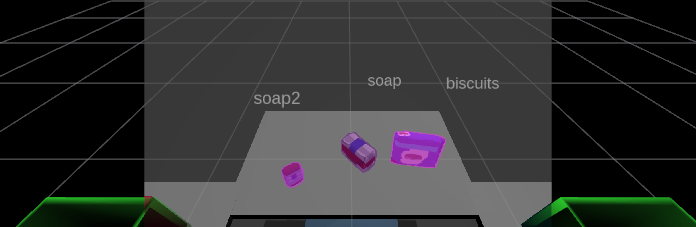
\includegraphics[scale=0.6]{test_case_1}}
	\caption{Test world one has three objects on the table, and \texttt{object\_recognition.py} correctly identifies 100\% of the items.}
\end{figure}

\subsection{Test World Two}
Test world two has five objects located on the table. The objects are a packet of biscuits, two different types of soap, a book, and some glue. The \verb|object_recognition.py| script correctly identifies all of the objects, except the book. The book is misclassified as snacks, meaning that only \%80 of the items are correctly classified. The \verb|pr2_mover()| function correctly outputs the required yaml file, which contains an error for the location of the book since it was unable to classify the object properly. The object recognition in operation can be seen in Figure 24. A YouTube video of the robot in operation can be found at the following link:
\begin{center}
	\url{https://youtu.be/E6hnXJOZiGc}
\end{center}

\begin{figure}[h]
	\centering
	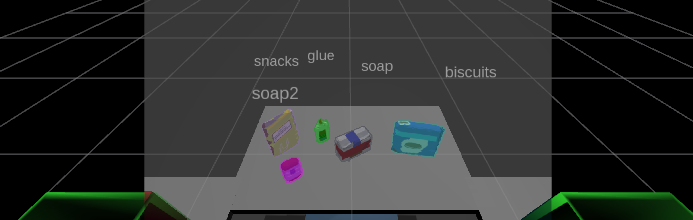
\includegraphics[scale=0.6]{test_case_2}
	\caption{Test world two has five objects on the table, and \texttt{object\_recognition.py} correctly identifies 80\% of the items.}
\end{figure}

\newpage
\subsection{Test World Three}
Test world two has five objects located on the table. The objects are sticky notes, a book, snacks, biscuits, an eraser, two types of soap, and some glue. The \verb|object_recognition.py| script correctly identifies all of the objects, except the book. The book is misclassified as snacks, meaning that only 87.5\% of the items are correctly classified. The \verb|pr2_mover()| function correctly outputs the required yaml file, which contains an error for the location of the book since it was unable to classify the object properly. The object recognition in operation can be seen in Figure 25. A YouTube video of the robot in operation can be found at the following link:
\begin{center}
	\url{https://youtu.be/5yA5dLXLfVs}
\end{center}

\begin{figure}[h]
	\centering
	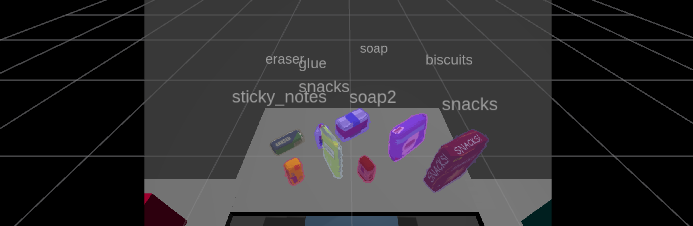
\includegraphics[scale=0.6]{test_case_3}
	\caption{Test world three has three objects on the table, and \texttt{object\_recognition.py} correctly identifies 87.5\% of the items.}
\end{figure}
%----------------------------------------------
\section{Results \& Conclusion}
The robot performed well in the segmentation section of the code filtering away the statistical noise, and separating the objects from the environment. Further, the robot correctly correctly assigned a set of points to each discrete object. The robot experienced some difficulty in the object recognition distinguishing between the snacks and the book. This may be due the similar shape, or more seriously, represent a shortfalling in the machine learning model chosen to perform object recognition. Despite this error, the robot was able to outperform the required benchmark outlined earlier: 100\% for test world one; 80\% for test world two; and 75\% for test world three.

%----------------------------------------------
\section{Further Enhancements}
To improve the object recognition a different machine learning model could be explored to provide more robust classification performance. Alternatively, there is the ability to modify the parameters for kernels such as rbf, or develop a custom kernel, which may improve the performance of the object recognition. Finally, it would be nice to have the robot pick and place each identified object, using either the left or right arm, however, this will be a future expansion of this project.
\clearpage

%----------------------------------------------
\section{Appendix A}
\lstset{
	frame=single,
	basicstyle=\ttfamily,
	numbers=left,
	showstringspaces=false,
}
The script used to capture feature data. The script works in conjunction with the ROS sensor stick environment in which the RGBD sensor for the PR2 robot is mounted on a stick. Gravity in the environment is disabled and the each object of interest is assigned random orientations in front of the sensor. RGBD point cloud data is captured for each of these orientations.
\tiny
\lstinputlisting[style=Python]{./code/capture_features.py}
\clearpage

%----------------------------------------------
\section{Appendix B}
\normalsize The script trains the Support Vector Machine using the feature and label data captured from the capture feature script shown in Appendix A. The trained model is saved for use with the PR2 robot object classification task.
\tiny
\lstinputlisting[style=Python]{./code/train_svm.py}
\newpage

%----------------------------------------------
\section{Appendix C}
\normalsize The function is called in the \verb|object_recognition.py| to output the yaml file in the directory from which the \verb|object_recognition.py| is run. 
\tiny
\lstinputlisting[style=Python]{./code/pr2_mover.py}
\end{document}